\section{Prüfstand und Versuchsdurchführung}
\label{sec:pruefstand}

Die Laufversuche dieser Arbeit wurden auf einem FZG-Kleinverspannungsprüfstand mit dem Achsabstand $52$\,mm gefahren. In der Semesterarbeit SA 1272 wurden zwei vorhandene Kleingetriebeprüfstände dieses Achsabstands für Laufversuche an nitrierten Zahnrädern mit dem Normalmodul $2$\,mm umkonstruiert. Der Grundaufbau folgt dem Verspannungsprüfstand der FZG in seiner Standardbauart, die nach Schurer in DIN 51354 genormt ist \cite[S.~2 und 8]{Schu09}. Übertragungsgetriebe und Prüfgetriebe sind über zwei Torsionswellen zu einem geschlossenen Leistungskreislauf verbunden. Das Prüfmoment entsteht durch Verdrehen und Verspannen der beiden Hälften einer Verspannkupplung und ist dem Verdrehweg proportional. Aufgebracht wird es mit einer Verspannschere oder mit einem Belastungshebel samt Gehänge und Gewichten. Der Motor speist nach dem Anlauf nur die Verlustleistung in den Kreislauf ein, die Ölversorgung übernimmt ein drucküberwachtes Ölaggregat, und ein Rohrheizkörper mit Schaltthermometer im Prüfgetriebekasten regelt die Schmierstofftemperatur \cite[S.~8]{Schu09}.

\figref{fig:pruefstand_sa1272} zeigt das Konstruktionsmodell des Prüfstands. Ein Servomotor mit einem Nennmoment von $7{,}6$\,Nm, mit Fremdlüfter etwa $12$\,Nm, treibt über eine Elastomerkupplung die Ritzelwelle des Übertragungsgetriebes. Dessen schrägverzahnte Räder übertragen die Leistung mit dem Zähnezahlverhältnis 29/21 auf die Radseite \cite[S.~9 und 48]{Schu09}. Die Radwelle des Übertragungsgetriebes läuft durch einen Lagerbock und ist über eine Kupplungshülse mit der Radwelle des Prüfgetriebes verbunden. Im Prüfgetriebe sitzen beide Wellen in einer Fest-Los-Lagerung aus Zylinderrollenlagern, und eine abnehmbare Frontplatte erlaubt den Wechsel der Prüfverzahnung \cite[S.~9 und 42]{Schu09}. Die Ritzelwelle des Prüfgetriebes führt in die Verspannkupplung, die wegen des kleineren Moments auf der Ritzelseite angeordnet ist und mit zwölf Verspannschrauben für $120$\,Nm am Ritzel ausgelegt wurde \cite[S.~46]{Schu09}. Zwischen Verspannkupplung und Übertragungsgetriebe liegt die Drehmomentmesswelle, die das Drehmoment mit Dehnungsmessstreifen erfasst und daneben Drehzahl und Wellenwinkel ausgibt; eine Balgkupplung bindet sie an die Ritzelwelle des Übertragungsgetriebes an \cite[S.~10 und 52]{Schu09}. Eine speicherprogrammierbare Steuerung im Schaltschrank steuert Prüfstand und Ölaggregat und gibt die Messwerte aus \cite[S.~53]{Schu09}. Als Prüfverzahnung sah die SA 1272 Stirnräder aus Nitrierstahl mit dem Normalmodul $2$\,mm bei den Zähnezahlen 21 und 29 vor; die Zahnbreite betrug $8$\,mm \cite[S.~42]{Schu09}. In dieser Arbeit läuft auf demselben Achsabstand die Prüfverzahnung kst-E mit dem Normalmodul $1$\,mm (\secref{sec:pruefverzahnung}). \Note{PH: Prüfstandsfoto.}

\begin{figure}[htbp]
    \centering
    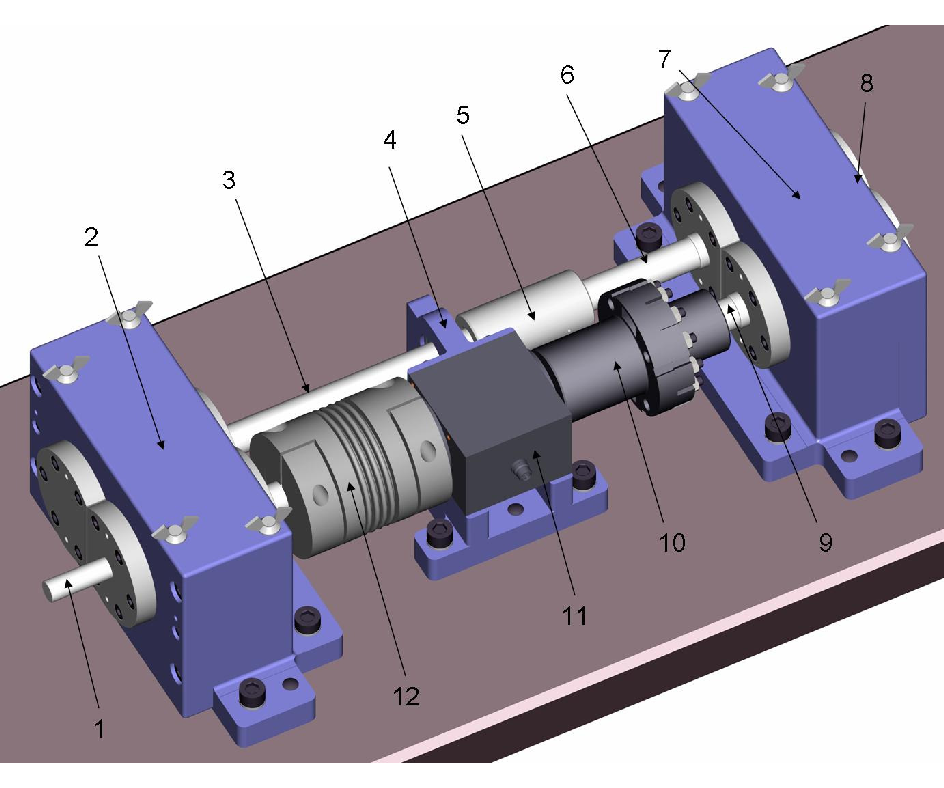
\includegraphics[width=0.8\textwidth]{kap3/quelle_pruefstand_sa1272}
    \caption{Verspannungsprüfstand mit dem Achsabstand $52$\,mm als Konstruktionsmodell: Ritzelwelle (1) und Übertragungsgetriebe (2), Radwelle (3) mit Lagerbock (4), Kupplungshülse (5), Radwelle (6) des Prüfgetriebes (7) mit Frontplatte (8), Ritzelwelle (9), Verspannkupplung (10), Drehmomentmesswelle (11) und Balgkupplung (12) auf der Grundplatte, nach \cite[S.~9]{Schu09}.}
    \label{fig:pruefstand_sa1272}
\end{figure}

Die Prüfbedingungen der Laufversuche an der kst-E-Verzahnung wurden für die Versuche des Jahres 2023 festgelegt \cite[S.~39 und 40]{Fie23}. Das Öl wird über Einlässe in den Deckeln der Getriebekästen zwischen die Zahnflanken eingespritzt und aus einer Bohrung im Kastenboden in den Kreislauf zurückgepumpt \cite[S.~10]{Schu09}; die Durchflussrate betrug $4{,}0$\,l/min. Schmierstoff ist das FVA-Referenzöl FVA 3A, ein Mineralöl der Viskositätsklasse ISO VG 100 mit $4$\,\% Anglamol 99. Die Prüfräder werden über den Schmierstoff temperiert, damit sich eine Zahnmassentemperatur von $80$\,°C einstellt. VDI 2736 Blatt 4 lässt bei Ölschmierung die Öltemperatur als Näherung für die Zahnfußtemperatur zu \cite[S.~16]{VDI2736-4}. Das Verspannmoment misst eine Drehmomentmesswelle burster 8651-5050-V0022 mit dem Messbereich bis $50$\,Nm im Verspannkreis. Auf der Welle sitzt das Kunststoffrad über eine Passfeder und ist mit einem Querpressverband gesichert, wozu der Lagerinnenring erwärmt und auf die mit Kältespray gekühlte Welle geschoben wird. Als Gegenrad diente 2023 ein einsatzgehärtetes Ritzel aus 16MnCr5 mit $20$\,\textmu m Kopfrücknahme \cite[S.~40]{Fie23}; das Ritzel dieser Arbeit ist in \secref{sec:pruefverzahnung} beschrieben.

Gegenüber den Versuchen 2023 blieben die Verzahnung, der Schmierstoff, die Einspritzschmierung und die Zieltemperatur von $80$\,°C unverändert. Die Versuche 2023 liefen auf dem Prüfstand KV4 mit dem Ritzel 86481 bei $2250$\,1/min. Für diese Arbeit läuft der Prüfstand KV3 mit dem Ritzel 95919 bei $3058$\,1/min am Ritzel, also $3000$\,1/min am Rad. \Note{PH: Zuordnung von KV3 und KV4 zu den beiden Exemplaren nach SA 1272 sowie Messwelle und Ölaggregat des KV3 bestätigen.} Während des Laufs kst-E\_72 wurde der Ölfilter gereinigt und der Durchfluss an einer neuen Düse auf $1{,}5$\,l/min eingestellt. \Note{PH: Öldurchfluss der Läufe 2026 vor dem Düsenwechsel.} Die Temperaturregelung bezieht sich auf den Prüfkasten, während das Ölaggregat im Dauerbetrieb etwa $10$\,K wärmer läuft; deshalb wird das Moment erst eingestellt, wenn sich beide Temperaturen angeglichen haben.

VDI 2736 Blatt 4 verlangt für die Ermittlung von Tragfähigkeitskennwerten Laufversuche bei festgehaltener Werkstofftemperatur, konstanter Drehzahl und konstantem Drehmoment bis zum Versagen des Bauteils \cite[S.~6]{VDI2736-4}. Je Paar aus Drehmoment und Temperatur sind mindestens drei Wiederholungen vorzusehen, für eine Temperatur mindestens vier Drehmomente \cite[S.~6 und 7]{VDI2736-4}. Die Versuche 2023 wurden als einstufige Wöhlerversuche auf drei Lastniveaus mit mindestens drei Versuchspunkten gefahren \cite[S.~65]{Fie23}. Dem folgt der Versuchsplan dieser Arbeit in \tabref{tab:versuchsplan}. Die Lasthorizonte sind als Radmoment $T_{\mathrm{2}}$ mit $8$\,Nm, $12$\,Nm und $16$\,Nm festgelegt; am Ritzel entspricht das über das Zähnezahlverhältnis 51/52 den Momenten $7{,}85$\,Nm, $11{,}8$\,Nm und $15{,}7$\,Nm. Als Drehzahl sind $3058$\,1/min am Ritzel eingestellt, als Öltemperatur $75$\,°C; die Zieltemperatur der Zähne beträgt $80$\,°C. Nach dem Wechsel des Temperatursensors am Prüfkasten und der Düse steht für die Läufe ab kst-E\_70 ein Sollwert von $67$\,°C in der Arbeitsmappe. Von den zehn Rädern der Kerngruppe diente 97351 dem Vorversuch kst-E\_63. Die übrigen neun Räder belegen die Horizonte: zwei Läufe bei $8$\,Nm (kst-E\_69, 75), drei bei $12$\,Nm (kst-E\_66, 68, 74) und vier bei $16$\,Nm (kst-E\_70 bis 73). \Note{PH: Rad des Laufs kst-E 75, Arbeitsmappe 97364 gegen Teileliste 97361.} \Note{PH: Stichtag der Laufversuche.}

\begin{table}[htbp]
    \caption{Versuchsplan der Laufversuche an der Prüfverzahnung kst-E nach der Arbeitsmappe des Prüfstands: Lasthorizonte dieser Arbeit (PA46-GF30, Prüfstand KV3, Ritzel 95919) sowie die Vergleichsläufe aus POM und PEEK auf demselben Horizont, 2026 auf demselben Prüfstand und 2023 auf dem Prüfstand KV4 (Ritzel 86481, $2250$\,1/min, Ritzelmoment $8$\,Nm, $12$\,Nm und $16$\,Nm, am Rad um 52/51 höher). Anzahl der Läufe PA46-GF30 als abgeschlossen/laufend mit den Teilenummern der Räder.}
    \label{tab:versuchsplan}
    \centering
    \footnotesize
    \setlength{\tabcolsep}{4pt}
    \begin{tabular}{L{1.6cm}L{1.6cm}L{1.5cm}L{1.6cm}L{2.3cm}L{1.1cm}L{1.1cm}L{1.1cm}L{1.1cm}}
        Moment Rad in Nm & Moment Ritzel in Nm & Drehzahl Ritzel in 1/min & Öl\-tempe\-ratur in °C & PA46-GF30 (Räder) & POM 2026 & PEEK 2026 & POM 2023 & PEEK 2023 \\
        \hline
        $8$  & $7{,}85$ & $3058$ & $74$ bis $75$ & 1/1 (97345, 97364) & 0 & 0 & 1 & 0 \\
        $12$ & $11{,}8$ & $3058$ & $74$ & 3/0 (97350, 97360, 97365) & 0 & 0 & 3 & 2 \\
        $16$ & $15{,}7$ & $3058$ & $67$ & 4/0 (97340, 97346, 97355, 97366) & 3 & 0 & 4 & 4 \\
        $8$, $12$, $16$ (Vorversuch) & $7{,}85$ bis $15{,}7$ & $2294$ und $3058$ & $75$ & 1/0 (97351) & & & & \\
    \end{tabular}
\end{table}

Der Vorversuch kst-E\_63 am Rad 97351 bestand aus einer Temperaturmatrix. Die drei Momente wurden mit den Drehzahlen $2294$\,1/min und $3058$\,1/min am Ritzel, also $2250$\,1/min und $3000$\,1/min am Rad, für je $2$\,h gefahren. Am Ende jeder Stufe wurde die Zahnflankentemperatur mit einem Infrarotthermometer bei dem Emissionsgrad $1$ gemessen. VDI 2736 Blatt 4 verlangt für optische Messungen den Emissionsgrad des Kunststoffs aus Voruntersuchungen und weist die Zuverlässigkeit des Verfahrens für Stirnräder als nicht nachgewiesen aus \cite[S.~17 und 18]{VDI2736-4}. Die Messwerte dienen deshalb dem Bezug auf die Zahnmassentemperatur von $80$\,°C in \secref{sec:temperatur} und nicht als Kennwert. Anschließend lief das Rad bei $3058$\,1/min bis zum Versagen weiter.

Jeder Lauf beginnt mit dem Verspannen im Stillstand. Das Moment wird mit dem Belastungshebel und Zusatzmassen an der Verspannkupplung aufgebracht, an der Messwelle abgelesen und mit einer Madenschraube gesichert. Der statische Wert liegt über dem Moment, das sich nach dem Start im Lauf einstellt. Eingetragen werden das Moment nach dem Start, nach $15$\,min und nach $60$\,min sowie der Stand des Lastwechselzählers der Steuerung. Fällt das Moment durch Verschleiß und Verformung der Kunststoffzähne ab, wird nachgespannt; VDI 2736 Blatt 4 fordert hierfür die Überwachung des Verspannmoments mit einer Drehmomentmessung \cite[S.~11]{VDI2736-4}. Bei den ersten Läufen geschah das bei Abfällen von etwa $1$\,Nm bis $3$\,Nm, teils mit Werten über dem Sollmoment. Ab dem Lauf kst-E\_74 gilt die Regel, nach $1$\,Nm Abfall auf höchstens $5$\,\% über dem Sollmoment nachzuspannen. Jedes Nachspannen wird mit Lastwechselzahl und Moment sowie den Temperaturen in der Spalte Bemerkung festgehalten, dazu der Befund einer Sichtprüfung der markierten Messzähne mit Fotos. Ein Lauf endet mit dem Zahnfußbruch, dessen Zahnnummer vermerkt wird, oder er läuft zum Stichtag noch.

Als Abbruchkriterium gilt der Totalausfall der Verzahnung, bei dem der Antrieb verloren geht. In den Versuchen 2023 zeigte POM ein schleichendes Risswachstum ohne eindeutigen Ausfallzeitpunkt \cite[S.~65]{Fie23}. Deshalb wurde dort zusätzlich ein Abfall des Drehmoments von mehr als $1$\,Nm über $100\,000$ Lastwechsel als Ausfall definiert, weil ab dieser Grenze keine zuverlässige Drehmomentübertragung mehr möglich ist. Dieses Ersatzkriterium wird in der Arbeitsmappe ab dem Lauf kst-E\_74 ausdrücklich übernommen. Ein zunehmendes sinusförmiges Laufgeräusch ist in den Bemerkungen als Vorzeichen des Bruchs festgehalten.

Auf demselben Prüfstand und mit demselben Ritzel fuhr die Betreuerin 2026 Vergleichsläufe mit Rädern aus POM und PEEK (kst-E\_50 bis 62, 64, 65, 67). Bei $3058$\,1/min und $75$\,°C Öltemperatur liegen drei POM-Läufe bei $16$\,Nm und drei bei $10$\,Nm am Rad, dazu drei PEEK-Läufe bei $14$\,Nm und vier bei $18$\,Nm. Drei weitere POM-Läufe bei $8$\,Nm liefen trocken bei Raumtemperatur und $1945$\,1/min und stehen außerhalb des Plans. \Note{PH: PEEK-Typ der Läufe 2026.} Die Läufe 2023 (kst-E\_1 bis 45) wurden auf dem Prüfstand KV4 mit dem Ritzel 86481 bei $2250$\,1/min mit Rädern aus POM (Delrin 100NC010) und PEEK (Vestakeep 4000G) gefahren \cite[S.~43 und 65]{Fie23}. Dort sind die Lastniveaus als Ritzelmoment von $8$\,Nm bis $18$\,Nm festgelegt und liegen am Rad um das Verhältnis 52/51 höher. Den Ritzelmomenten $8$\,Nm, $12$\,Nm und $16$\,Nm entsprechen am Rad $8{,}16$\,Nm, $12{,}2$\,Nm und $16{,}3$\,Nm. In den Vergleich gehen die Läufe bei $73$\,°C bis $76$\,°C Öltemperatur und $2250$\,1/min ein. Außerhalb bleiben die ersten sieben Läufe mit $45$\,°C Öltemperatur, zwei Stufenläufe, die Läufe bei $1000$\,1/min bis $4000$\,1/min sowie die ohne Rad eingetragenen Zeilen.

% Herkunft:
% Absatz 1 (Prüfstand, Prinzip): SA-1272.txt S. 2 (Aufgabenstellung: zwei vorhandene Kleingetriebeprüfstände a = 52 mm,
%   Grundaufbau wie Standard-FZG-Verspannungsprüfstand), S. 8 (DIN 51354, geschlossener Leistungskreislauf, zwei
%   Torsionswellen, Verspannkupplung, Verdrehweg proportional, Verspannschere oder Belastungshebel mit Gehänge und
%   Gewichten, Motor speist Verlustleistung, drucküberwachtes Ölaggregat, Rohrheizkörper mit Schaltthermometer, zwei
%   Modelle gefertigt). Druckseite = PDF-Seite.
% Absatz 2 (Bauteile): SA-1272 S. 9 (Bild 2, Nummern 1 bis 10, Motor ca. 12 Nm, Elastomerkupplung, i = 29/21, Lagerbock,
%   Kupplungshülse, Frontplatte, Verspannkupplung mit Verspannschere), S. 10 (Messwelle 11, dämpfende Kupplung 12,
%   Grundplatte 13, Einspritzung über Einlässe in den Deckeln, Bohrung im Boden), S. 42 (4.3.4 Tabelle 1: a = 52, z 21/29,
%   mn 2, b 8, Nitrierstähle 31CrMoV9 und 15CrMoV5.9; 4.3.5 Fest-Los-Lagerung, Zylinderrollenlager), S. 43 (NUP204/NU204),
%   S. 44 bis 46 (Verspannkupplung zweiteilig, Verspannschrauben, auf der Ritzelseite, 12 Schrauben, 120 Nm am Ritzel),
%   S. 48 (KEB-Servomotor D3.SM.000.4400, 7,6 Nm bei 4000 1/min, mit Fremdlüfter ca. 12 Nm), S. 51 (Balgkupplung R&W
%   BKH150/95), S. 52 (Burster-Messwelle 100 bzw. 200 Nm, DMS, Drehzahl und Wellenwinkel, auf dem Lagerbock), S. 53
%   (Schaltschrank, SPS Simatic S7-300 steuert Ölaggregat und Prüfstand, Messwerterfassung). Modul 1 mm heute: Verweis
%   auf sec:pruefverzahnung.
% Absatz 3 (Prüfbedingungen 2023): MA-0296.txt Z. 1913 bis 1961 (PDF S. 52/53 = Druckseiten 39/40, Seitenoffset 13):
%   a = 52,0 mm, Öldurchfluss 4,0 l/min, burster 8651-5050-V0022 bis 50 Nm, Einspritzschmierung, Temperierung über
%   den Schmierstoff auf 80 °C Zahnmassentemperatur, Ritzel 16MnCr5 einsatzgehärtet mit 20 µm Kopfrücknahme,
%   Querpressverband (Passfeder, Lagerinnenring erhitzt, Welle mit Kältespray gekühlt), FVA 3A = FVA-Referenzöl Nr. 3,
%   ISO VG 100, 4 % Anglamol 99 (Tabelle 3). Öltemperatur als Näherung der Zahnfußtemperatur: VDI2736-4.txt Z. 1056
%   bis 1062, Abschnitt 8.2.2, Druckseite 16 (vor dem Kopf "– 17 –" in Z. 1082).
% Absatz 4 (gleich/anders): kst-E_Laufversuche_KV3.xlsx Blatt Tabelle1: Spalten Prüfstand (KV4 Zeilen 2 bis 52, KV3 ab
%   Zeile 53), ME-Nr. Ritzel (86481 bei 2023, 95919 bei 2026), Drehzahl (2250 bei 2023, 3058 bei den Läufen 2026 ab
%   kst-E_53); 3058 · 51/52 = 2999,1 1/min; Ölfilter gereinigt und 1,5 l/min an neuer Düse: Bemerkung kst-E_72 (Zeile 94);
%   Prüfkastentemperatur gegen Aggregattemperatur etwa 10 K, Moment erst nach dem Angleichen einstellen: Bemerkung
%   kst-E_71 (Zeile 93). KV4 auch in MA-0296 Druckseite 84 (Z. 3325) genannt.
% Absatz 5 (Versuchsplanung): VDI2736-4.txt Z. 365 bis 371 (Abschnitt 3, Druckseite 6: festgehaltene Materialtemperatur,
%   konstante Drehzahl, konstantes Drehmoment, Lastwechsel bis zum Versagen), Z. 380 bis 386 (3.1, S. 6: mindestens eine
%   Temperatur, mindestens vier Drehmomente, Block mit mindestens drei Wiederholungen), Z. 449 bis 455 (3.3, S. 7, n_wi >= 3);
%   dasselbe in Abschnitt 4, Z. 562 bis 568 (Druckseite 9, Kopf "– 9 –" in Z. 557), im Text nicht zitiert; MA-0296 Druckseite 65 (Z. 2780
%   bis 2786: einstufige Wöhlerversuche, 3 Lastniveaus mit mindestens 3 Versuchspunkten). Horizonte: xlsx Spalte
%   "Ziel Drehmoment Ritzel" 7,9 bzw. 7,8 / 11,8 / 15,7 Nm und Spalte "Drehmoment Rad" = Ritzel · 52/51 (8,05 bzw. 7,95 /
%   12,03 / 16,01 Nm); nachgerechnet 8 · 51/52 = 7,846, 12 · 51/52 = 11,769, 16 · 51/52 = 15,692 Nm. Drehzahl 3058,
%   Öltemperatur 75 (kst-E_63, 75), 74 (66, 68, 69, 74), 67 (70 bis 73), Ziel/Zahntemperatur 80: Zeilen 77 bis 95.
%   Sensorwechsel: letzte Spalte der Zeilen 91 bis 94 ("Durch Änderung des Temperatursensors beim Prüfkasten, andere
%   Düse, und womöglich zu wenig Volumenstrom"). Belegung: Zeile 77 kst-E_63 97351; 88 kst-E_66 97350 (12 Nm);
%   90 kst-E_68 97365 (12); 91 kst-E_69 97345 (8); 92 kst-E_70 97346 (16); 93 kst-E_71 97366 (16); 94 kst-E_72 97355
%   (16); 95 kst-E_73 97340 (16); 96 kst-E_74 97360 (12); 97 kst-E_75 97364 (8, Lastwechsel leer, läuft).
%   Kerngruppe: parts.yaml groups.core (97340, 97345, 97346, 97350, 97351, 97355, 97360, 97361, 97365, 97366).
% Tabelle: Zahlen wie Absatz 5; Vergleichsläufe 2026 (Zeilen 53 bis 89): POM kst-E_54, 55, 56 bei 15,7/16,0 Nm, 3058,
%   75 °C; POM kst-E_53, 57, 67 bei 9,8/10,0 Nm; PEEK kst-E_61, 62, 65 bei 13,73/14,0 Nm; PEEK kst-E_58, 59, 60, 64 bei
%   17,7 bzw. 17,65/18,0 Nm; POM kst-E_50, 51, 52 bei 7,9/8,05 Nm trocken, RT, 1945 1/min (ausgeschlossen); Zeilen 72
%   bis 75 sind Doppeleinträge der Läufe 58 bis 61 ("Daten verlieren wegen Problem von Rechner"), nicht gezählt.
%   Vergleichsläufe 2023 (Zeilen 2 bis 46, Ritzelmoment = Spalte "Ziel Drehmoment Ritzel", Rad = · 52/51):
%   8 Nm POM kst-E_40; 12 Nm POM kst-E_14, 15, 21 und PEEK kst-E_24, 42 (kst-E_30 vorzeitig abgebrochen,
%   "weiterführbar", ohne Lastwechsel, nicht gezählt; kst-E_22 Stufenlauf, nicht gezählt); 16 Nm POM kst-E_12, 19, 20, 29
%   (29 ohne Drehzahleintrag) und PEEK kst-E_11, 25, 26, 37 (kst-E_43 Stufenlauf, nicht gezählt; kst-E_6 bei 45 °C
%   Öl, nicht gezählt). Ausgeschlossen: kst-E_1 bis 7 (Öl 45 °C), 28/32/33/34/35/39 (3000, 4000, 1000 1/min),
%   44/45 (ohne Datum und Rad). 8 · 52/51 = 8,157, 12 · 52/51 = 12,235, 16 · 52/51 = 16,314 Nm.
% Absatz 6 (Vorversuch): xlsx Zeilen 77 bis 83 (kst-E_63, 97351: 11,8/2294, 11,8/3058, 7,9/2294, 7,8/3058, 15,7/2294,
%   15,7/3058, jeweils "nach 2h ... Zahnflankentemperatur mit Emissionsgrad 1 (nach Test von Liang)"; Zeile 83:
%   Weiterlauf bei 3058 bis "5-6 kaputte Zähne"); 2294 · 51/52 = 2249,9 1/min. Emissionsgrad und Zuverlässigkeit:
%   VDI2736-4.txt Z. 1097 bis 1123 (8.2.4, Druckseite 17) und Z. 1145 bis 1148 (Druckseite 18). Temperaturwerte selbst
%   nicht genannt (Kapitel 4.5, Label sec:temperatur aus kap4_voruntersuchungen.tex).
% Absatz 7 (Ablauf): xlsx Spalten "verspannt", "Drehmoment Ritzel T_0 nach Start", "15 min", "T / 60 min",
%   "T_nachgespannt", "Lastwechsel", "Bemerkung"; Hebel mit Masse und Madenschraube, statisch 14,9 gegen dynamisch
%   12,4 bis 12,5 Nm: letzte Spalte kst-E_74 (Zeile 96) und Bemerkung kst-E_69 ("Hebel 1,2 Nm mit Masse 8,7 Nm
%   statisch"); Nachspannregel "nach 1 Nm Drehmomentabfall ... max +5 % Drehmomentabweichung vom Sollmoment":
%   letzte Spalte kst-E_74; frühere Läufe mit Abfällen von 1 bis 3 Nm und Werten über dem Soll: Bemerkungen kst-E_66
%   (8,9 auf 12,8 bis 13,0 Nm), 68 (auf 13,1 bis 13,3 Nm), 70 (auf 17,1 bis 17,2 Nm); Sichtprüfung der markierten
%   Messzähne mit Fotos: Bemerkungen kst-E_69, 74, 75; Zahnnummer in der Spalte Versagensart (Zeilen 91 bis 95);
%   Verschleiß und Verformung als Ursache des Abfalls und Überwachung mit Drehmomentmessung: VDI2736-4.txt
%   Z. 726 bis 731 (5.2, Druckseite 11).
% Absatz 8 (Abbruchkriterium): MA-0296.txt Z. 2787 bis 2793 und Abbildung 53 (PDF S. 78 = Druckseite 65): Totalausfall
%   "Loss-of-drive", schleichendes Risswachstum bei Zahnfußbruch, zusätzlich Abfall des Drehmoments von mehr als 1 Nm
%   über 100 000 Lastwechsel; Übernahme ab kst-E_74: letzte Spalte Zeile 96 ("Als Abbruchkriterium Totalausfall ...
%   Ersatzausfallkriterium"); sinusförmiges Geräusch: Bemerkungen kst-E_69, 73, 74.
% Absatz 9 (Vergleichsläufe): 2026 wie bei der Tabelle, Versuche der Betreuerin laut Auftrag; 2023: xlsx Zeilen 2 bis 46
%   (KV4, 86481, 2250), Werkstoffe MA-0296 PDF S. 56 = Druckseite 43 (POM-H Delrin 100NC010, PEEK Vestakeep 4000G),
%   Druckseite 65 (Versuchsprogramm); Ritzelmoment als Lastangabe: MA-0296 nennt 8, 12, 14, 16, 18 Nm (z. B. Druckseite
%   66, Tabelle 9 "12 Nm"), die xlsx führt diese Werte in der Spalte "Ziel Drehmoment Ritzel".
% Bildwunsch: kap3/quelle_pruefstand_sa1272 aus SA-1272_Schurer_unlocked.pdf, Druckseite 9 (= PDF-Seite 9), Bild 2
%   "3D-Modell des fertigen Prüfstandes" mit den Nummern 1 bis 13 (Beschreibung S. 9 und 10); Ausschnitt das ganze Bild
%   ohne die Bildunterschrift. Ersatz, falls das Modellbild zu klein gedruckt ist: Druckseite 8, Bild 1 "Schematische
%   Skizze des Standard-FZG-Zahnrad-Verspannungsprüfstandes" (dort nach [5], [10] der SA, also Sekundärbild).
% Bildwunsch (Nutzer): Foto des Prüfstands KV3 (PH im Text, keine figure-Umgebung angelegt).
% Bibwunsch: keine neuen Einträge; Schu09, Fie23 und VDI2736-4 stehen in litbib.bib. <SCRATCH>\bib_kap3_2.bib bleibt leer.
% Nomenklatur: T_2 (Drehmoment am Rad, N m) steht als T mit Index 2 in Nomenklatur.tex; n (1/min) steht dort. Keine
%   neuen Zeichen; Temperaturen und Emissionsgrad ohne Formelzeichen genannt.
% Offen:
% - Rad des Laufs kst-E_75: die Arbeitsmappe (Zeile 97) nennt 97364 bei 7,8 Nm Ritzel (8 Nm Rad, laufend); parts.yaml
%   und kap3_1 (Tabelle Teilegruppen) führen 97361 als laufendes Rad bei 8 Nm und 97364 als Zusatzversuch bei 12 Nm der
%   Streugruppe. 97361 kommt in der Arbeitsmappe nicht vor. Entweder Tippfehler in der Mappe oder parts.yaml falsch.
% - Fehlerfenster Zähne 36 bis 40 (parts.yaml failure_window, kap3_3): die Spalte Versagensart nennt Zahn 34 (kst-E_69),
%   Zahn 40 und 41 (70), Zahn 31 (71), Zahn 39 (72), Zahn 40 (73); kst-E_68 und 74 "ZFB" ohne Zahnnummer. Drei der
%   fünf Nummern liegen außerhalb des Fensters. Im Text 3.2 wird das Fenster deshalb nicht genannt.
% - kst-E_66 (97350, 12 Nm): Versagensart leer, Lastwechsel eingetragen; als abgeschlossen gezählt.
% - Drehzahl 2250 der Läufe 2023: die Arbeitsmappe und MA-0296 sagen nicht, ob Ritzel oder Rad gemeint ist; 2026 ist
%   2294 am Ritzel = 2250 am Rad eingestellt.
% - Öldurchfluss der Läufe 2026 vor der neuen Düse (4,0 l/min nach MA-0296 oder anders) und Messwelle des KV3 unbelegt.
% - Datum kst-E_66 (2026-08-18) gleich dem Datum des Vorversuchs; nicht übernommen.
